\part{Towards Highly Miniaturized LED Power Systems }
\label{ch:twrd_HMLED}

\chapter[LEDification]{LEDification: Transition towards LED lighting }


The light bulb is one of the most relevant inventions from our past history. Electrical lighting was definitely a revolution in the early 19${th}$ century society; for the first time in history people had a clear, reliable and safe source of artificial light was embedded in a single device easy to distribute and control. The apparition  of the electrical light bulb was also, without doubt, the trigger for the commercialization of electric power and the deployment of the first power distribution networks~\cite{14NYISO}. The impact was to such a degree that it settled two capital sectors of the present industry, the lighting and the electric power distribution, with  world recognized companies such as Philips, General Electric and Osram.  Actually, both sectors have been so close related that often we use the word \emph{light} when we actually mean \emph{electricity}. In short, a single invention changed our society forever, bringing light and electricity to our homes.

\begin{figure}[!h]
\centering
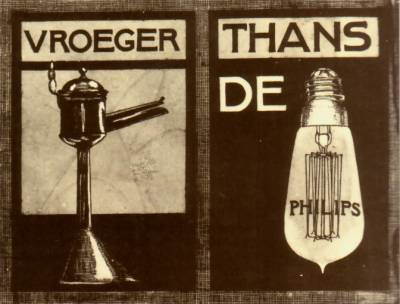
\includegraphics{./0_intro/img/1900-philips3.jpg}
\caption[Philips lights advertisement from 1900]{Philips advertisement from 1900 comparing what was before -\emph{Vroeger}, an oil lamp- and now -\emph{Today, the} incandescent light bulb~\cite{lib:Philips}.}
\label{fig:incandescent_light_blub}
\end{figure}


From the initial invention of the first incandescent light bulb onwards, important research has continuously been done to improve the most important characteristic of the incandescent light bulb, the efficacy. Incandescent light bulbs are extremely inefficient at generating light, with a luminous efficacy between $12.6 lm/W$ for a tungsten incandescent bulb, and  up to $24 lm/W$ for a quartz halogen lamp (see Table~\ref{tab:lighting_tech}). In a more comprehensive way, we can say that in general incandescent lights convert just at most 5\% of the supplied energy in light and at least 95\% in heat. Knowing that lighting represents 17\% of world energy consumption, we can account that 15\% of the world's consumed power is transformed to heat and only 1.7\% is transformed real light \footnote{Estimated values for the year 2008}. Although generating heat is not intrinsically negative, specially for spaces that have to be heated, the propose of a light is to illuminate the space in the most efficient meaner; that is why there is a motivation and necessity to improve the efficacy/efficiency of light bulbs.

\begin{SCfigure}[][!h]
\centering
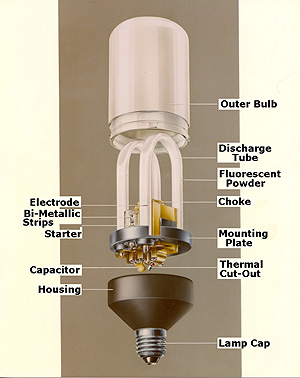
\includegraphics{./0_intro/img/phil1b.jpg}
\caption[Compact fluorescent lamp]{Exploded view of Philips SL the first compact fluorescent lamp launched to the market~\cite{lib:Philips}.}
\label{fig:philips_sl}
\end{SCfigure}

Gas-discharge lamps were one of the first alternatives for incandescent lamps that proved a better efficacy, with the fluorescent tub the most popular in this family. The low pressure mercury-vapor gas-discharge  lamp, commonly called \emph{fluorescent}, was probably on of the first relevant innovations in the lighting industry~\cite{39inman}. Initially the tubes where mainly used for the interior lighting of industrial buildings, offices, schools and similar~\cite{39oDay,82bouwknegt}, and after, in the late 1980's, started populating households with the appearance of the \emph{compact fluorescent lamps}\footnote{Screw-in version of a fluorescent tube. Currently you can find a CFL replacement for almost the majority of sockets in the market.} (CFLs)~\cite{82bouwknegt}, being currently the market standard for energy efficient light bulbs~\cite{11EPA}; as shown in Figure~\ref{fig:philips_sl}. Fluorescent lamps are indeed a big improvement in efficacy with respect to the incandescent lamps. The luminous efficacy ranges between 52-100 $lm/W$ depending on the color rendering index (CRI), converting about 22\% of the input power to visible light. More details of other gas-discharge bulbs are presented in Table~\ref{tab:lighting_tech}. Notwithstanding the better efficiency of the CFLs, due to the following reasons they have not yet fully replaced the inefficient incandescent ones~\cite{11EPA}:

\begin{itemize}
  \item Standard CFLs are not dimmable.  Dimmable CFLs are more expensive, their behavior is not standardized among manufacturers, producing mismatches in the light output between lamps, what does not satisfy consumer's desires.

  \item CFLs have a slow warm-up time\footnote{Gas-discharge lamps have to be warm in order to volatilise and mix chemical elements that compose the gas. Depending on the chemical elements this process can take from a minute up to ten minutes. }. Not being suitable for places where lights are turned on for short times.

  \item CFLs have unappealing form and look. Some can not fit in existing fixtures that mount incandescent lamps. The \emph{pig tail} appearance is not attractive when bulbs are exposed.

  \item The low price of the incandescent light bulb compared to a CFL is more attractive for the consumer. Although CFLs save more money due to power savings, the end consumers are still repelled by the retail price of the lamps.

\end{itemize}
Therefore, in 2012, it was estimated that in residential environments more than 50\% of the installed light bulbs were still incandescent ~\cite{13ALED}. Showing still the need for a another lighting technology capable of replacing the old inefficient incandescent lamps.

\begin{figure}[!h]
\centering
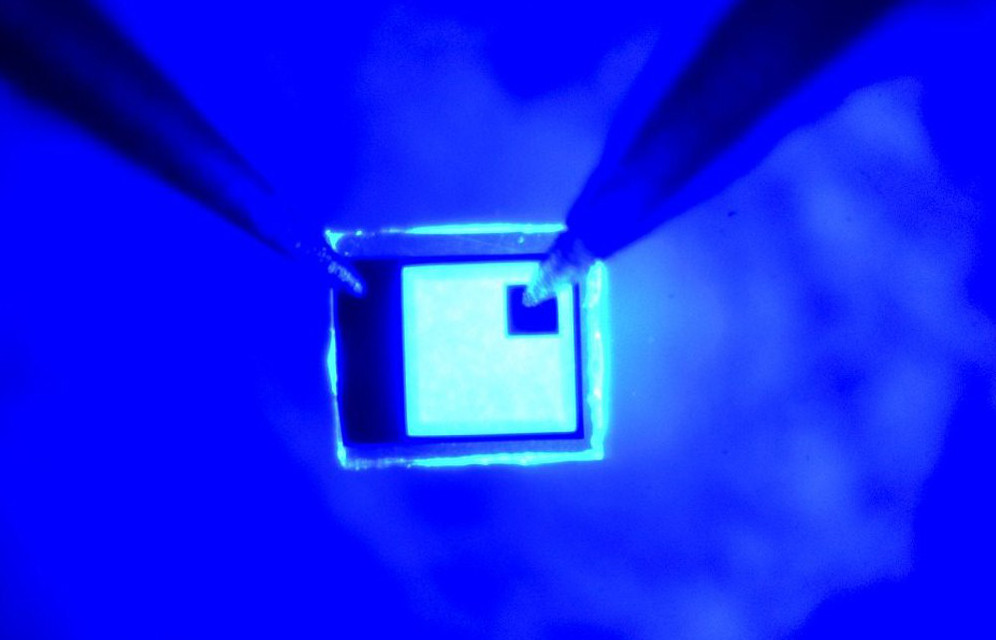
\includegraphics[width=4cm]{./0_intro/img/10-7-14-nobel-prize-blue-led.jpg}
\caption{Bare die of a working blue LED  .}
\label{fig:blue_LED}
%\caption*{Source: \url{http://www.newsweek.com/how-blue-led-changed-world-and-won-nobel-prize-275977} }
\end{figure}

Actually the bases of one potential new technology were settled  in 1994, with the invention of the high-efficiency blue \emph{light-emitting diode} (LED) by Sush Nakamura's ~\cite{94Nakamura}, shown in Figure~\ref{fig:blue_LED}. A subsequent finding after the initial work of Isamu Akasaki and Hiroshi Amano~\cite{94akasaki}, where it was  demonstrated that was possible to generate blue light from semiconductor materials. Blue light is fundamental to generate withe light for LED lamps~\cite{02narukawa}. Both findings were key steps in the transforation of the artificial lighting towards the solid state lighting (SSL), with such an important relevance that they were awarded with the 2014 Nobel prize in physics~\cite{14NobelPhy}

The advantages of SSL are:
\begin{description}
  \item [Efficiency] The light generation inside a LED is the direct mechanism of hole-electron recombination. The supplied energy is better used compared to an incandescent lamp. The power consumption can be up to an order of magnitude lower than an incandescent light.

  \item [Size] LEDs are tiny and flat devices, which can be considered as 2-D elements,  and do not need any vacuum chamber to work. They are much more flexible in the assembly process and can easily replace the old glass-based bulb design.

  \item [Color] LED light has a very narrow light spectrum that can be used to produce colored light directly. Colored lights are growing in popularity in households, becoming a decoration piece or mood tweaking device.

  \item [Dynamics] Compared to any of the traditional sources of light, LEDs have no dynamics. Actually they have, but they are so fast that cannot be tracked by the human eye. They do not have any setting time when turned on, contrary to the CFLs. Their fast dynamics allow to modulate the light and even transmit data without disturbing human beings~\cite{2000Tanaka,2004Komine}.

  \item [Lifetime] Solid State devices do not wear out, therefore they can be considered to have an infinite lifetime. In practice LEDs make use of organic phosphores, thus the light quality degrades over used time. The practical life expectancy of the LED is rated from 20.000 - 100.000 hours, 20 to 100 times longer than the life expectancy of the classical light bulbs. In order to take advantage of this long life, the different elements of lighting systems must be properly designed otherwise the lamps can experience a short life~\cite{2005Narendran}.
\end{description}

Just looking at the benefits that LEDs offer LED in terms of efficiency, the projected energy savings for 2020 are $297TWh$ only in USA. The \emph{United States Environmental Protection Agency}~\cite{14USDoE} published that reducing the household lighting energy consumption by half - easy to achieve by using LED lighting -  more than \$13 billion a year in energy costs could be saved, more than 80 million metric $CO_2$ tones would be avoided each year, % and the need for over 30\footnote{To be further detailed} power plants could be eliminated.
The advantages of LED lamps are so relevant that the \emph{United States National Lighting Bureau}~\cite{14USDoE} forecasts a market penetration growth from 5\% in 2015, to 74\% in 2020 and reaching 88\% in 2030, as shown in the graph of Figure~\ref{fig:lighting_forecast}. Hence in the near future almost all lighting technology will be LED based.

The transition towards LED based lighting technologies, referred as \emph{LEDification}~\cite{13Hammerschmidt,15crawford}, is predicted to come in two waves~\cite{13liedenbaum}. The first wave will be a replacement period. The main focus will be to bring fast and simple LED technology in form of light to the consumers in order to remove the inefficient old lighting technologies. The second wave will include more intelligence to the light fixtures, transforming the lights from a simple light sources to connected nodes within an infrastructure of interconnected lights, what is already crystalizing with \emph{The Connected Lighting Alliance}. This second phase is predicted to be a revolution, transforming  the lighting infrastructure into a crucial element of the future smart houses and in the internet-of-things era~\cite{14Harbers}. Therefore LED lighting will bring not only efficient lighting, but also interconnect light fixtures. This is similar to what happened before, in the late 1800s, when a single invention brought simultaneously light and electricity to our homes~\cite{14NYISO}.

\begin{figure}[!h]
\centering
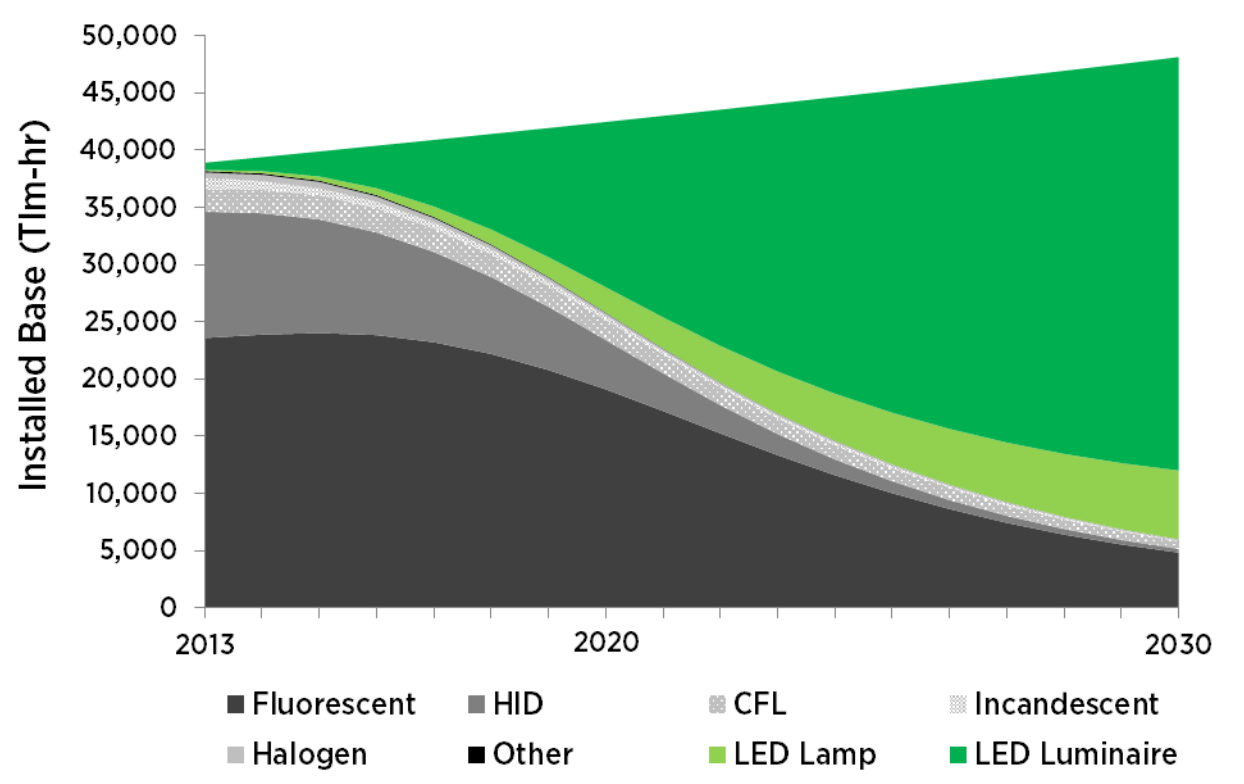
\includegraphics[width=10cm]{./0_intro/img/lighting_forecast.png}
\caption{U.S. Lighting Service Forecast, 2013 to 2030~\cite{14USDoE}.  }
\label{fig:lighting_forecast}
\end{figure}

During the last decade, the lighting industry has been in a rush to bring LED light to the market, making \emph{LEDification} a reality. Initially LED lighting was only used for decorative lights and with the advance of the LED technology with higher efficiency devices, they started to be applied in general lighting applications. With the progression of efficiency of the LEDs, in May 2008 the U.S. Department of Energy (DOE) established the Bright Tomorrow Lighting Prize (L-Prize)~\cite{web:LPrize,09Taub} competition in order to encourage the industry to spur development of ultra-efficient SSL products awarded with US\$10 million cash prize. In the L-Prize competition the industry was challenged to develop replacement technologies for two most widely used and inefficient bulbs: \emph{A19 60W} incandescent lamps and \emph{PAR38} halogen lamps.

On September 2009, Philips Lighting North America became the fist to submit LED lamps in the category to replace the standard 60W screw-in lamps, becoming the winer in that category~\cite{web:Winer-LPrize,web:Wright}; the other category is still empty. Only three years later, in 2012, Philips had already covered the whole range of incandescent bulbs up to 100W~\cite{13liedenbaum}. Today in 2015, all these replacement lamps are available in almost all of the supermarkets and retail shops, although they are not yet adopted as the preferred solution by consumers. Despite of the advantages of LED lighting, end consumers are still very reluctant to make the change towards SSL products due to their elevated price~\cite{11Voger,15Greig}. Currently a 100W LED replacement costs between \$20 - \$40 compared to less than \$3 for an halogen incandescent. The reason for this is because the majority of end consumers do not yet understand that even incandescent lamps are cheaper, LED replacements save money over the life time of the product due to energy savings. With the help of Table \ref{tab:lighting_tech} we can easily demonstrate this  statement.

The \emph{Lumen cost of owner ship}\footnote{Lumen cost of owner ship is expressed in $klm/$€ indicating how many lumens you can produce per € during thousand hours. Using this metric the different light technologies can be compared independently of the lamp power consumption.} for incandescent technologies is below 60 $klm/$€ and for LED technologies is easily above 200$klm/$€. Translating these figures to total costs\footnote{Lamp amortization are included in the costs}, it is estimated that in a productive year (around 2000$h$), for a 25$ m^2 $  office space\footnote{Recommended illumination for productive office spaces is 500$ lm/m^2 $}, costs of lighting would be above 420€ for incandescent lamps and below 140€ for LED lamps. It is true that linear fluorescent and \emph(High-Intensity Discharge Sodium) (HID-SON) represent the best option regarding costs below 80€, but the projected performance gains in efficacy, color quality and light distribution point that LED technology will be come the best choice~\cite{14Braga}. HID-SON lamps are out of discussion since they  have a very poor CRI (25) what does not allow to properly recognise colors. Based on the aforementioned facts is predicted that LED is going to be the future lighting technology~\cite{13Uken,14USDoE}, but still the industry has find the manner to motivate the end consumers to buy LED lamps as their first choice~\cite{11Voger}.


\begin{landscape}
\thispagestyle{empty}
\begin{table}[h]

\centering
\caption{Characteristics for different lamp technologies (winter 2015).}
\label{tab:lighting_tech}
\renewcommand{\arraystretch}{1.5}% Wider
\begin{tabular}{l | r |  *{10}r }
% after \\: \hline or \cline{col1-col2} \cline{col3-col4} ...
\mcrot{1}{l}{60}{} & \mcrot{1}{c}{0}{Units} & \mcrot{1}{c}{60}{Incandescent}  & \mcrot{1}{c}{60}{Halogen} &  \mcrot{1}{c}{60}{Cold-White Fluorescent} & \mcrot{1}{c}{60}{Warm-White Fluorescent}& \mcrot{1}{c}{60}{Compact Fluorescent} & \mcrot{1}{c}{60}{HDI SON} & \mcrot{1}{c}{60}{Retrofit LED Budget } & \mcrot{1}{c}{60}{Retrofit LED Dimmable } & \mcrot{1}{c}{60}{Retrofit LED} & \mcrot{1}{c}{60}{Retrofit Tube LED}  \\
  \midrule

  Power                     & $W$            & 100   & 53    & 36    & 39    & 11    & 70    & 10    & 13    &  5  & 10.5  \\
  Flux                      & $lm$           & 1203  & 845   & 3100  & 3100  & 600   & 5600  & 600   & 1055  &   350  & 950   \\
  Efficacy                  & $lm/W$         & 14.3  & 14.42 & 57.14 & 57.14 & 55    & 80    & 60    & 81.15 &    70  & 90.5  \\
  Color Temperature         & $K$            & 2700  & 2800  & 4000  &  3000 & 2700  & 2000  & 2700  & 2700  &  3000  & 3000  \\
  Color Rendering Index     &                & 100   & 100   &   85  &  85   &  82   &  25   & 87    & 80    &  80    & 85    \\
  Lifespan                  & $h$            & 1000  & 2000  & 20000 & 24000 & 15000 & 28000 & 2500  & 25000 & 15000  & 50000 \\
  Retail price              & €          & 1     & 3     & 5.6   & 4.8   & 8.78  & 14.26 & 4.5   & 37.1  & 17     & 43    \\
  Lumen cost of ownership   & $ klmh/$€ & 48    &   59  & 348   & 324   & 186   & 324   & 233    & 229   &  182   & 281   \\
  Cost of ownership         & €$/kh$     & 25    &  14.2 & 8.9  & 9.6   & 3.2   &  17.3 & 2.6    &  4.6  &  3.3   & 3.4   \\
  Cost for a 20$m^2$ office & €$/kh$     & 260    & 210 & 36     & 39    & 67     & 39  &  54   &  55    & 69     & 43 \\
%  \hline
\end{tabular}
\end{table}
\end{landscape}

\vspace{5mm} %5mm vertical space


\begin{SCfigure}[][!h]
\centering
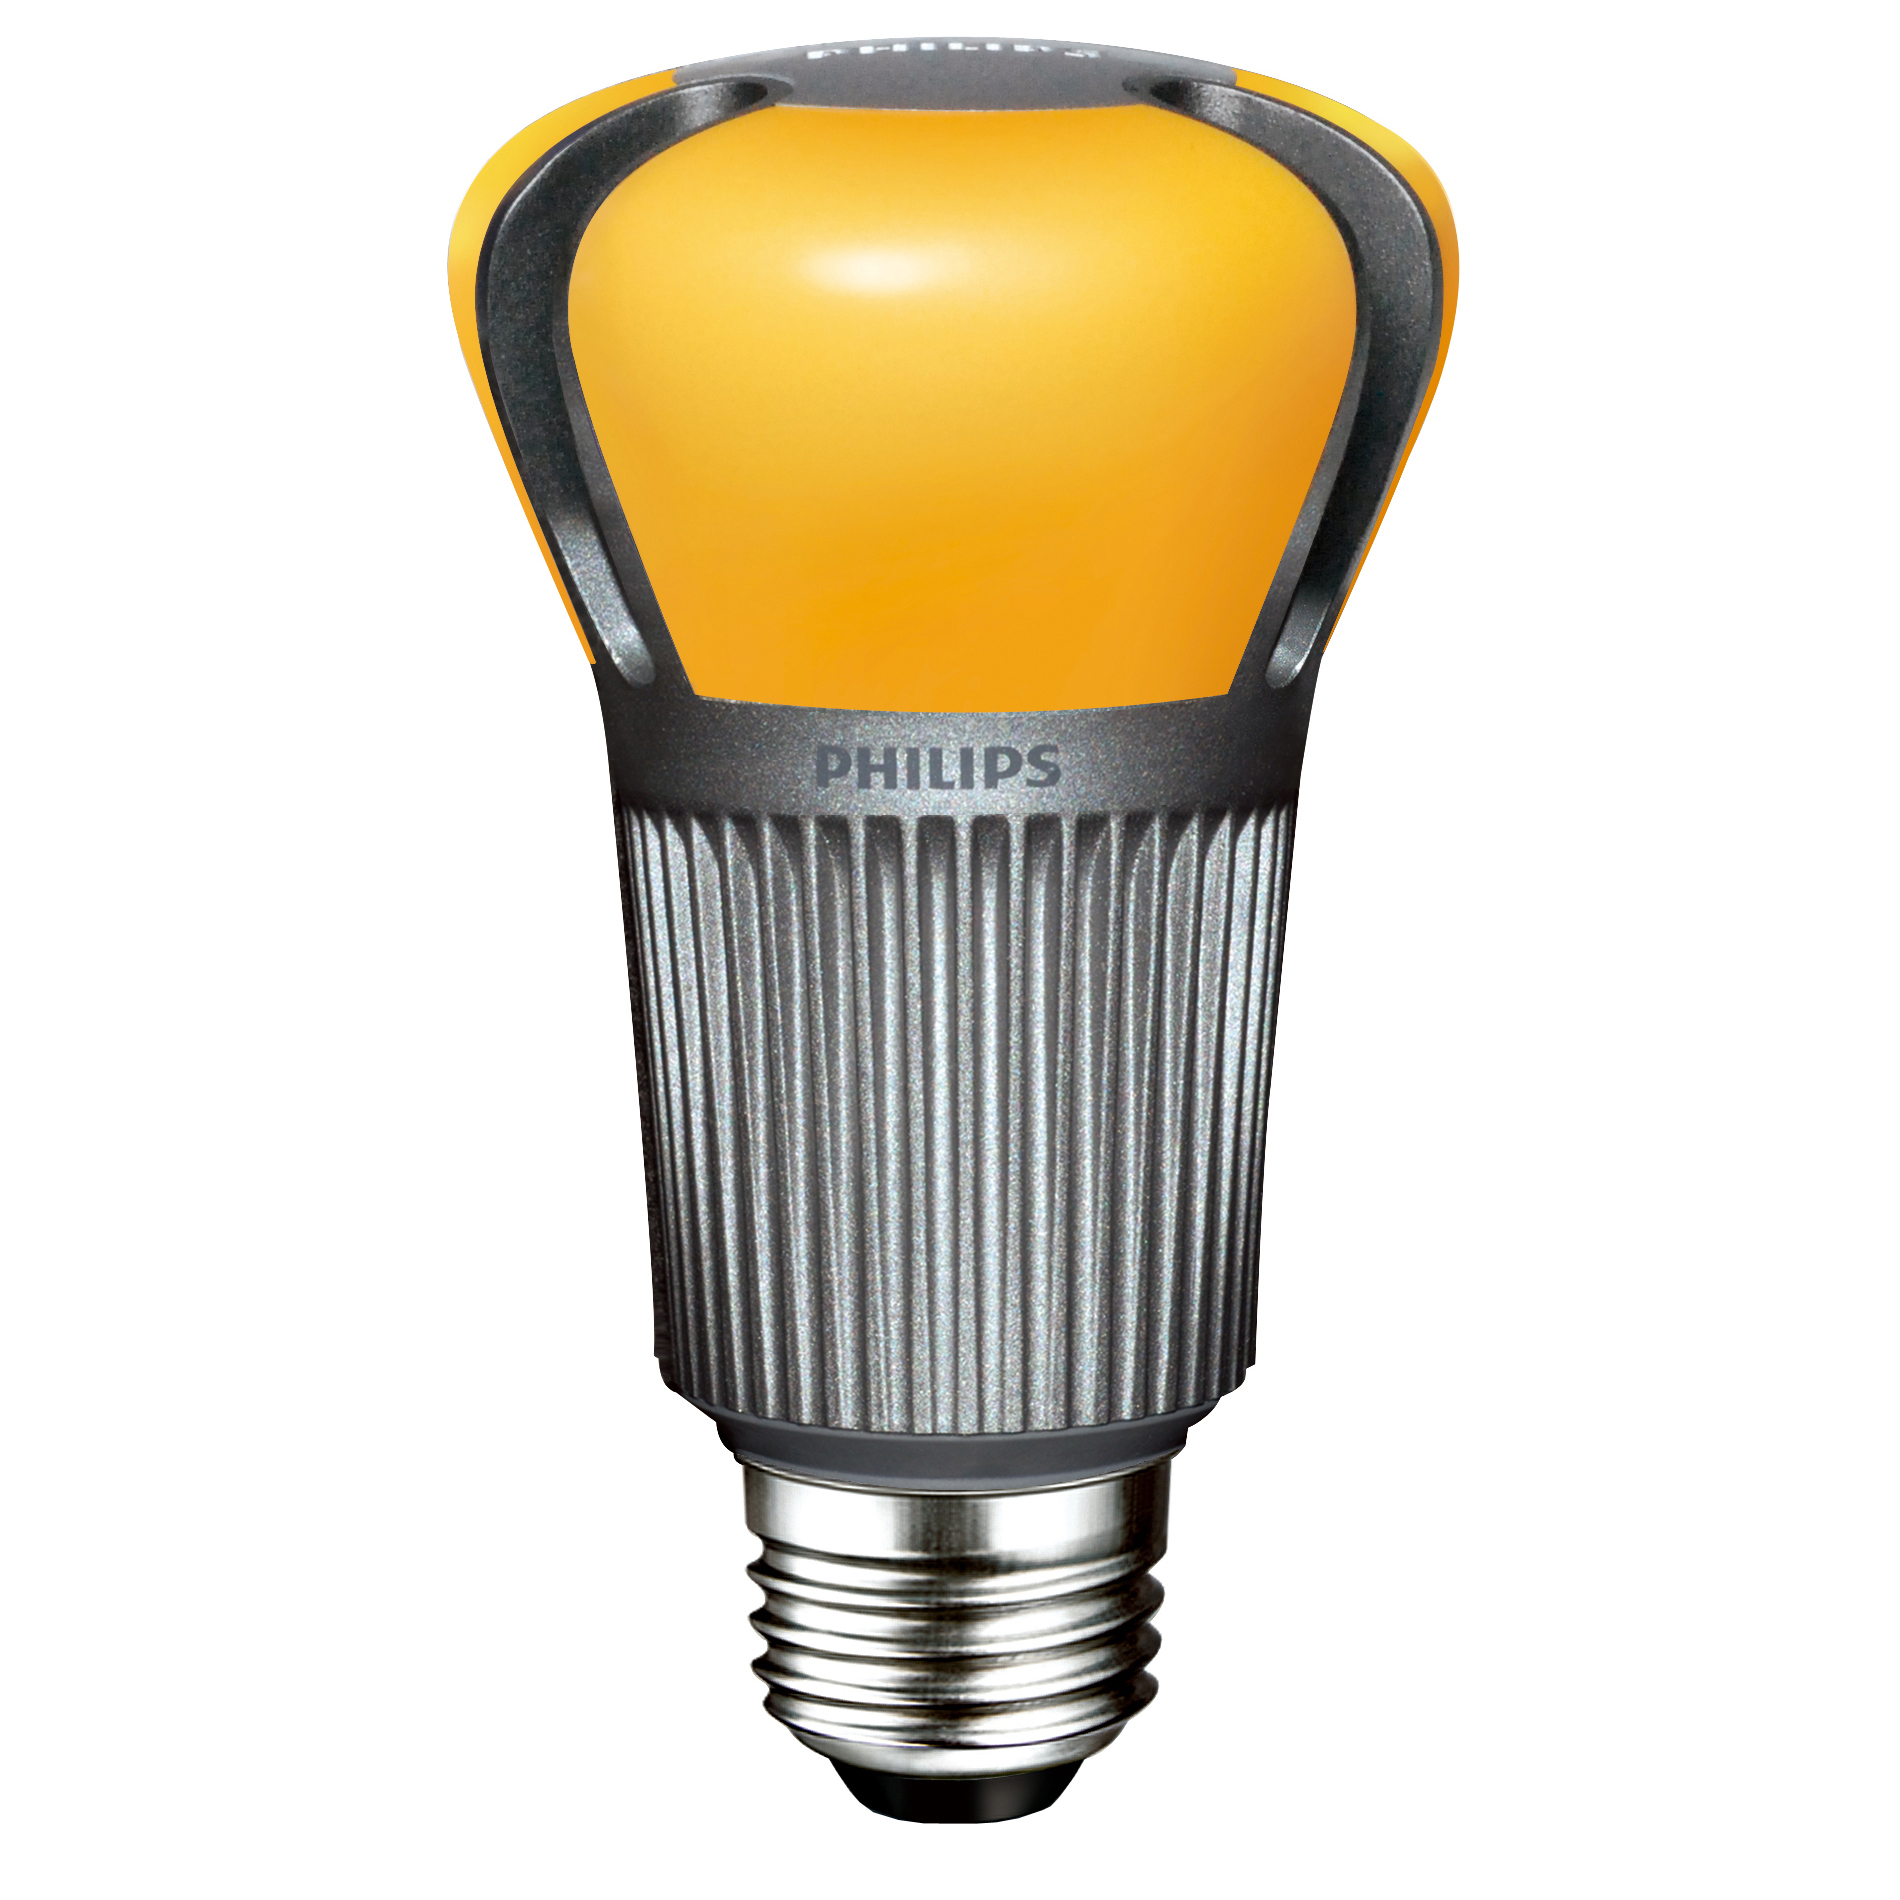
\includegraphics[width=4cm]{./0_intro/img/enduraled-12w.jpg}
\caption{900 lumens LED light bulb.}
\label{fig:l_prize}
\end{SCfigure}

Two main factors have been identified to help the adoption of LED as the preferred lighting solution for consumers~\cite{11Voger}. First, reducing the end product price; second, bringing more value than traditional lighting sources. Certainly, as previously mentioned, LED light bulbs already bring more value compared to the old light bulbs. They are much more efficient, almost one order of magnitude lower in power consumption, and have a longer lifetime, easily twenty times more operating hours. However, that is not yet well explained to be a valuable argument for the end consumers. New \emph{smart} bulbs concepts are starting to populate the market, such as LIFX, Philips Hue and Easybulb, offering color tuning, light output dimming, remote control and other wireless services. This position SSL in line with the current trend of the \emph{internet-of-things}~\cite{03Qiu,atzori2010internet,weber2010internet}, for the specific lighting case, the \emph{internet-of-lights}~\cite{14Harbers,web:14Harbers}. Moreover, LED lighting is also growing the luminaries industry, bringing more and more popular products where the light fixture directly embeds the LEDs. Providing products which benefit from design advantages enabled by the small form factors of the LEDs. As a matter of fact the \emph{U.S Department of Energy} (U.S.DoE) estimates that LED luminaries will be the big player in the lighting market, shown in the graph of Figure ~\ref{fig:lighting_forecast}.

Generally the market penetration of SSL is identified to be influenced by three main factors:
\begin{itemize}
  \item End lamp/luminaire price
  \item Intelligence: Interactivity, connectivity and controllability\
  \item Light fixture size: Luminaire design, shape and application
\end{itemize}

It is necessary to describe the different elements in an LED lamp in order to relate this three factors with current LED bulbs and understand the challenges in their development. The system can be grouped in six main elements described below and shown in  the Figure~\ref{fig:exploded_bulb}.

\begin{description}
  \item[LED] From its acronym, a \emph{Light-Emitting Diode}  is a two-lead semiconductor device that generates light when a current flows through it. Internally light is produced by the electroluminescence effect, where an electron recombines with an electron-hole releasing energy in form of photons. The color of the light is determined by the energy band gap of the semiconductor. The mounted LEDs in the lamp will determine light color, power, efficiency and load characteristics.

  \item[Optics] Optical device that mixes and distributes the light from the LED to the illuminated space.

  \item[Driver] Electronic circuit designed to transform the electrical power of the input source to properly supply the LEDs. LED drivers are considered voltage-to-current($v-i$) power supplies.  The driver control the current through the load, hence the light output, being the active part of the system that essentially controls the lamp.

  \item[Heat sink] Mechanical element that acts as a passive heat exchanger to cool the hot elements inside the lamp by dissipating the heat into the surrounding medium. In the LED bulb the energy that is not transformed to light becomes heat and must be extracted from inside the lamp. The hot spots areas in the lamp are the LEDs chips and some of the driver components.

  \item[Body assembly] Mechanical element that hold alls the different subsystems in one single device. In many cases the heat sink is also served for that propose.

  \item[Connector] Mechanical element that provides connection with the energy source. The most popular one is the Edison connector present in all screw-in lamps. There are many other popular ones, such as GU10, MR16, MR11, coming from the halogen multifaceted reflector bulbs, or the 2-pin connector of the fluorescent tubes.

      In many cases, the standardized connectors restrict the mechanical design of the lamp. Their old-fashioned design is not optimal for the new lamps.
\end{description}

With an understanding of the different elements of a LED lamp we can relate them back to the three factors that influence the market penetration previously mentioned. First, the price of the lamps. Figure~\ref{fig:cost_breakdown} shows the cost breakdown for different lighting applications. The three main elements Driver, LED package and Thermal/Mechanical/Electrical interface\footnote{The Thermal/Mechanical/Electrical group comprises the heat sink, socket connector and \emph{Printed circuit Boards} (PCBs) that interconnect and mount the input socket, LEDs and driver.} share  almost equally the costs of the lamp, and it is predicted to be similar or even a bit better distributed as shown in the forecast of Figure~\ref{fig:cost_breakdown_forecast}. Based on these figures, it is evident that in order to achieve the predicted cost reduction, one half for 2020, actions have to be started at the system level, ensuring an equal research and development effort for all elements in the lamp.

\begin{figure}[!h]
\definecolor{LED}{HTML}{AA3939}
\definecolor{TEM}{HTML}{582A71}
\definecolor{DRV}{HTML}{FF8500}
\definecolor{OPT}{HTML}{0D59C2}
\definecolor{ASB}{HTML}{7BA833}
\definecolor{OVH}{HTML}{295475}

\centering
\begin{subfigure}[t]{.45\textwidth}
    \raggedright
    \begin{tikzpicture}
        \begin{axis}[
            width=\textwidth,
            ybar stacked,
        	bar width=18pt,
           % nodes near coords,
            ylabel = { \% },
            ylabel near ticks,
            y label style={font=\tiny},
        	axis y line*=left,
            axis x line*=bottom,
            ymin=0,
            ymax=100,
            symbolic x coords={
                Outdoor,
                Downlight,
                A19 Lamp},
            xtick=data,
            x tick label style={rotate=0,anchor=north, font=\tiny},
            y tick label style={rotate=0,anchor=east, font=\tiny},
            legend style={
                legend columns = 6,
                at={(1.3,1.075)},
                anchor=south,
                draw=none,
                font=\tiny,},
            y tick style={draw=none},
            x tick style={draw=none},
        ]
        \addplot+[LED,fill=white, postaction={pattern=north east lines}] plot coordinates
        {(Outdoor,20) (Downlight,33) (A19 Lamp,35)};
        \addplot+[TEM,fill=TEM] plot coordinates
        {(Outdoor,40) (Downlight,30) (A19 Lamp,30)};
        \addplot+[DRV,fill=DRV] plot coordinates
        {(Outdoor,17) (Downlight,20) (A19 Lamp,15)};
        \addplot+[OPT,fill=OPT] plot coordinates
        {(Outdoor,5) (Downlight,5) (A19 Lamp,10)};
        \addplot+[ASB,fill=ASB] plot coordinates
        {(Outdoor,3) (Downlight,4) (A19 Lamp,5)};
        \addplot+[OVH,fill=OVH] coordinates
        {(Outdoor,15) (Downlight,8) (A19 Lamp,5)};

        \legend{LED, Electrical, Driver, Optics, Assembly, Overhead}
        %\legend{\strut never, \strut rarely, \strut sometimes, \strut often}
        \end{axis}
    \end{tikzpicture}
    %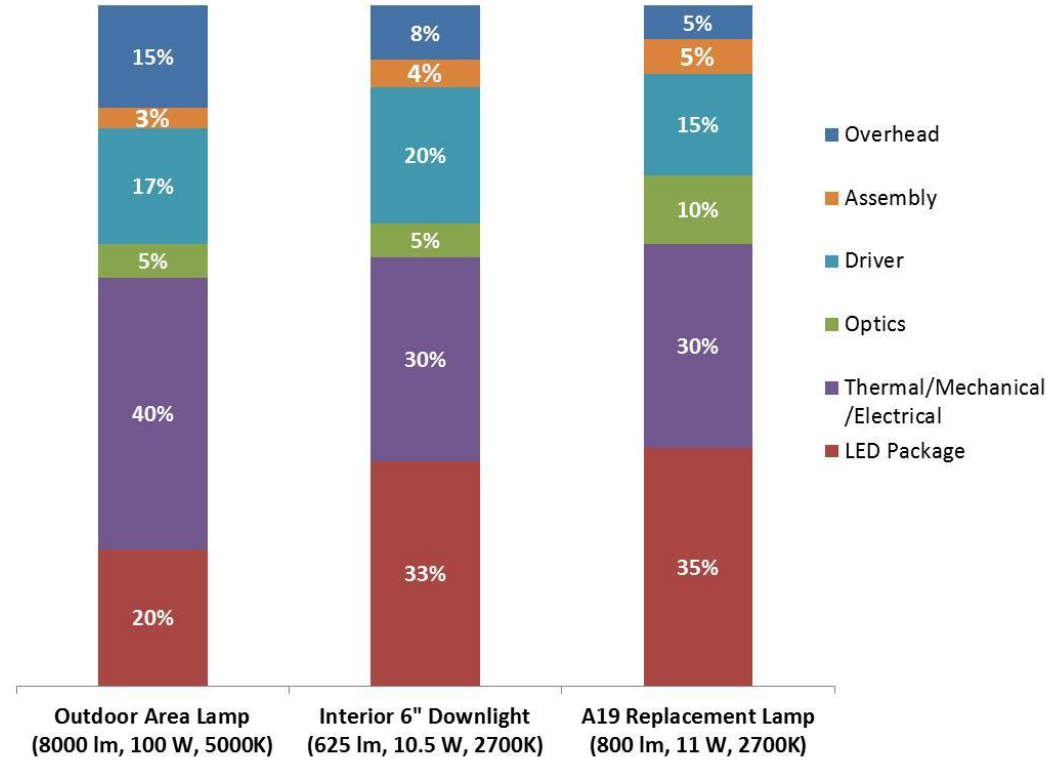
\includegraphics[width=\textwidth]{./0_intro/img/cost_breakdown.png}
    \caption{}
    \label{fig:cost_breakdown}
\end{subfigure}
\begin{subfigure}[t]{.45\textwidth}
   \raggedleft
   %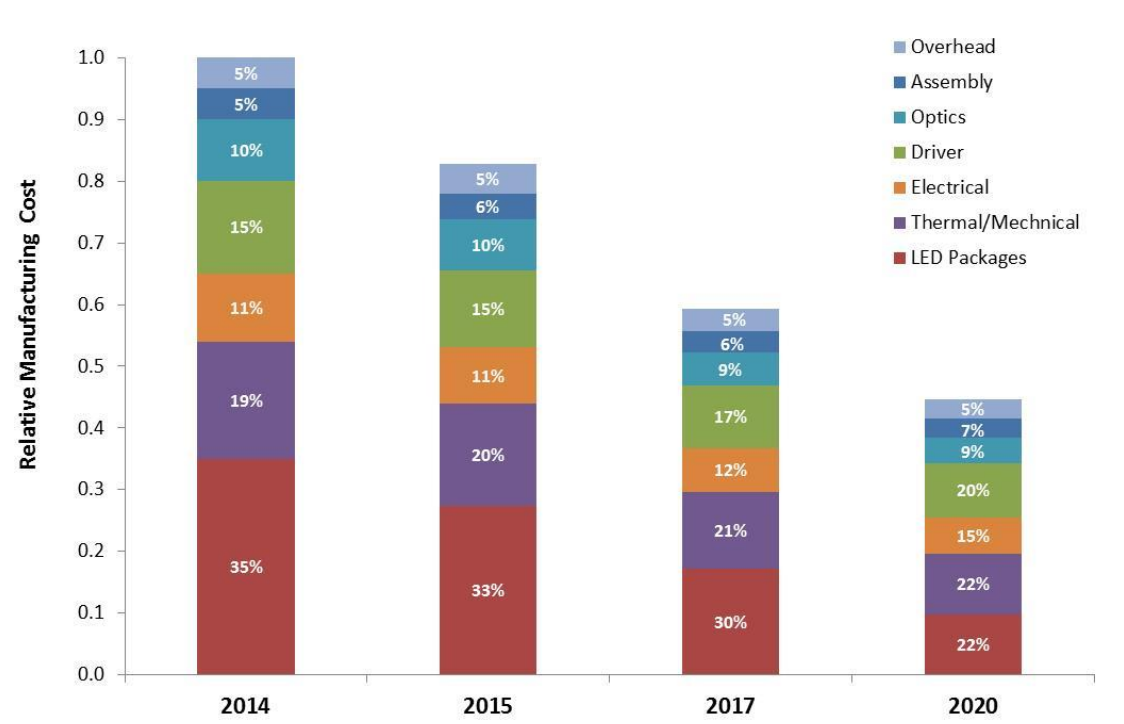
\includegraphics[width=\textwidth]{./0_intro/img/cost_breakdown_forecast.png}
   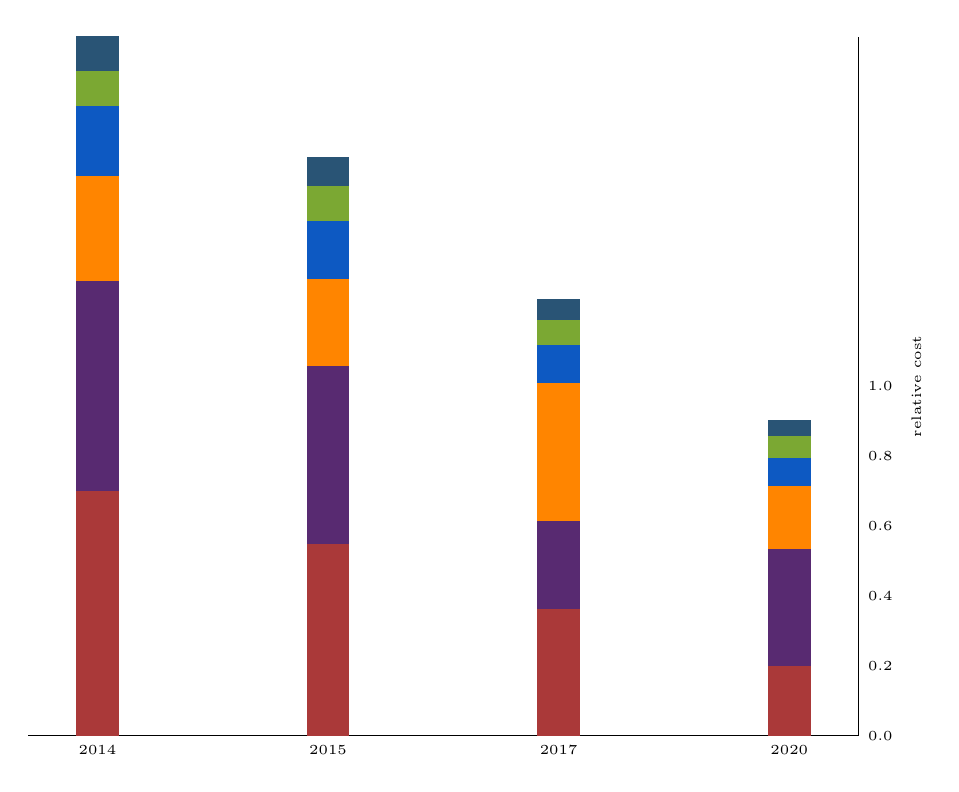
\begin{tikzpicture}
        \begin{axis}[
            width=\textwidth,
            ybar stacked,
        	bar width=15pt,
           % nodes near coords,
            ylabel = {relative cost},
            ylabel near ticks,
            y label style={font=\tiny},
            axis y line*=right,
            axis x line*=bottom,
            ymin=0,
            ymax=100,
            symbolic x coords={
                2014,
                2015,
                2017,
                2020},
            xtick=data,
            x tick label style={rotate=0,anchor=north, font=\tiny},
            y tick label style={rotate=0,anchor=west, font=\tiny},
            y tick style={draw=none},
            x tick style={draw=none},
            yticklabels={0,0.0, 0.2, 0.4, 0.6, 0.8,1.0},
        ]
        \addplot+[LED,fill=LED] plot coordinates
        {(2014,35) (2015,27.3) (2017,18) (2020,9.9)};
        \addplot+[TEM,fill=TEM] plot coordinates
        {(2014,30) (2015,25.6) (2017,12.6) (2020,16.7)};
        \addplot+[DRV,fill=DRV] plot coordinates
        {(2014,15) (2015,12.4) (2017,19.8) (2020,9)};
        \addplot+[OPT,fill=OPT] plot coordinates
        {(2014,10) (2015,8.3)  (2017,5.4) (2020,4.1)};
        \addplot+[ASB,fill=ASB] plot coordinates
        {(2014,5) (2015,5)     (2017,3.6) (2020,3.15)};
        \addplot+[OVH,fill=OVH] coordinates
        {(2014,5) (2015,4.1)   (2017,3) (2020,2.25)};



        \end{axis}
    \end{tikzpicture}
   \caption{}
   \label{fig:cost_breakdown_forecast}
\end{subfigure}
\caption[Breakdown costs and forecasts in LED lighting]{\emph{Left}-Comparison of cost breakdown for different lighting applications; \emph{right} - Cost breakdown projection for a typical A19 replacement lamp\\
\emph{Source: DOE SSL Roundtable and Workshop attendees}}
\label{fig:costs_BD_FC}
\end{figure}

%\begin{figure}[!h]
%    \centering
%    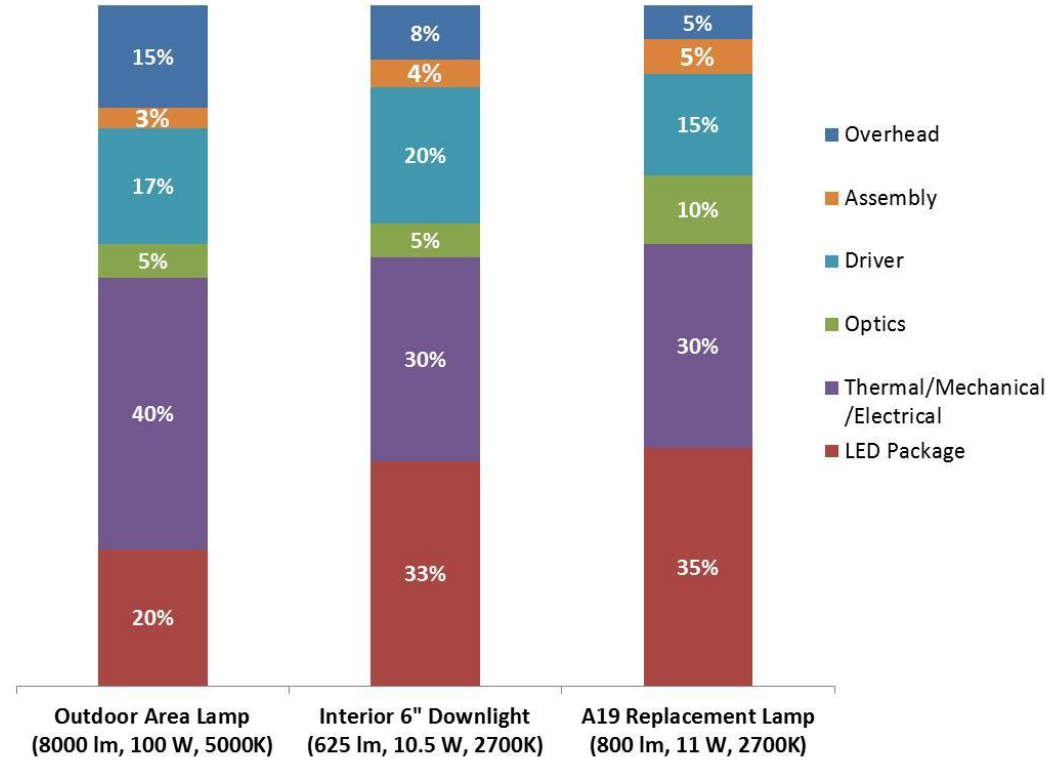
\includegraphics[width=.85\textwidth]{./0_intro/img/cost_breakdown.png}
%    \caption{Comparison of cost breakdown for different lighting applications\\
%            \emph{Source: DOE SSL Roundtable and Workshop attendees}}
%    \label{fig:cost_breakdown}
%\end{figure}
%
%\begin{figure}[!h]
%   \centering
%   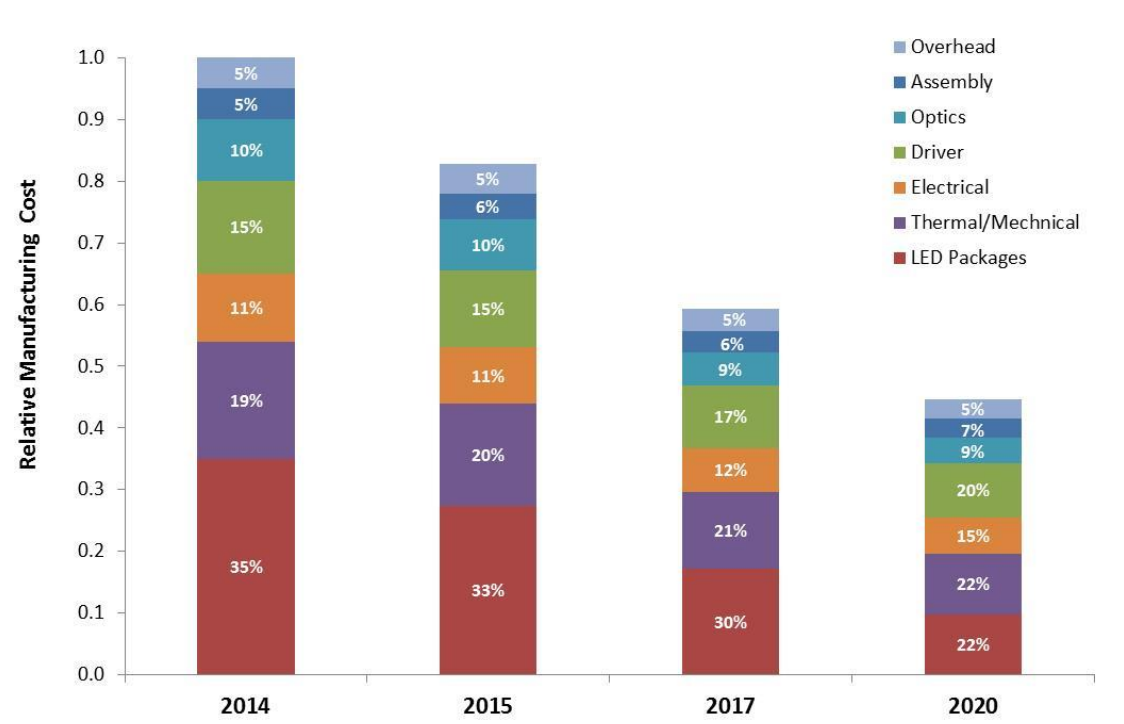
\includegraphics[width=.85\textwidth]{./0_intro/img/cost_breakdown_forecast.png}
%   \caption{Cost breakdown projection for a typical A19 replacement lamp \\
%            \emph{Source: DOE SSL Roundtable and Workshop attendees}}
%   \label{fig:cost_breakdown_forecast}
%\end{figure}

The LEDs or LED package \footnote{Electronic part composed by an assembly of LEDs connected in series or parallel and mounted on a single substrate} are in continuous evolution in order to fit the requirements of the luminarie manufacturers and driver requirements in terms of price, efficacy and package. Innovations are on the market with three available technologies based on current capability of the dies: low, mid and high power range. The different offer in chip packages brings more flexibility at the system level in terms of optical design, luminarie light projection, color, and driver design. However full potential of the reduced profile of the LED has not yet been explored in regard to the luminaire design. Further research at the die level will improve the reliability of manufacturing process, and the efficiency needed to reduce the costs of the lamps. It is, however, in the better use of the small size of the LED what will provide more value for the future lamp designs and competitions like \emph{Next Generation Luminaires} (\url{http://www.ngldc.org/}) challenge the industry to innovate in that field.

\begin{figure}[!h]
    \centering
    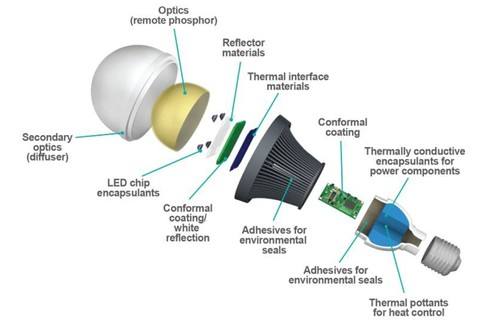
\includegraphics[width=8cm]{./0_intro/img/exploded_bulb_2.jpg}
    \caption{Exploded vision of an LED light bulb.}
    \label{fig:exploded_bulb}
\end{figure}


The Mechanical/Thermal/Electrical group - comprising heat sink, socket connector, PCBs and \emph{Electromagnetic Interference} (EMI) filters - still plays a dominant role in the design of the lamp. The heat sink and the connector are in many cases the body of the lamp where the heat sink and assembles form the entire lamp. Traditional sockets, which are not design friendly, are currently kept in order to provide a fast transition for the current first wave of the \emph{LEDification}, the replacement period. Replacement lamps are also known as \emph{retrofit}\footnote{Adding the new LED technology to the older light bulb systems. In that way the end user can directly replace an old lamp or tube by a LED one without needing to make any change in the current installation.} lamps. The current offer of \emph{retrofitted} LED bulbs proves the successes achieved in that area. Nowadays is already possible to find a replacement lamp for almost all old lamps. However \emph{retrofitted} lamps will have only an small market share as predicted in the lighting forecast of Figure~\ref{fig:lighting_forecast}. That is why innovations in the Mechanical/Thermal/Electrical group will be necessary for the coming light fixtures, to evolve and reinvent the future LED luminaries, where the small size, the low profile and the colored light of the LEDs will play an relevant role.


The driver is, with no doubt, the most \emph{special} component of the entire lamp. It is referred to as \emph{special} because it is the only element of the lamp that plays a role in each of the three factors of influence for market penetration: Intelligence, Design and Costs. First, the driver is the only element that brings active functionality to the lamp, hence the only one that can incorporate the control and interactivity to the system. Second, its volume and its location influence the design of the lamp. The closer the driver to the LEDs is, the better the controllability and the intelligence of the system becomes. Finally, the manufacturing costs, what up-to-now has been the main research interest for LED drivers.

For the past years cost down reduction has enabled to bring the prices for simple \emph{retrofitted} lamps down to competitive levels. However the chosen circuit architectures for low cost drivers are very cost sensitive towards more intelligent drivers, as it can be seen with the different prices for the \emph{dimmable}, \emph{non-dimmable} and \emph{smart} lamps of  Table~\ref{tab:lighting_tech}. That is why a different approach in the driver architectures must be taken in order to respond to the challenges for the future intelligent and connected LED lamps. In other words, the driver architecture that will provide power management, intelligence and connectivity together, assembled in a reduced volume, and at low cost will be, with no discussion, the key element to carry the future of LED lighting technology.

The current driver architectures are based on discrete implementations. In such an approach driver circuits are composed by different discrete components all assembled on a single \emph{printed-circuit-board} (PCB), which enables a fast development and cheap costs, because the mounted parts are general propose components sold by millions; however this approach has several limitations. First the performance of old and cheap components limits the volume reduction of the required  passive components in the drivers filters and magnetics. Second, as the circuit increases in complexity, the \emph{bill of materials} (BOM) and there fore the costs increases, also the costs, therefore reducing the possibilities to offer more functionality in the driver circuit, such as connectivity and controllability at reduced costs. In resume, fulfilling the driver requirements for the second generation of LED lamps will be very challenging using  discrete driver  architectures.

The approach to meet the requirements for the future lamps will probably rely on an integrated driver solution; meaning by integrated an \emph{application-specific integrated circuit} or ASIC. This approach from the perspective of the integrated power supplies brings the focus of the research to drivers where the power converter can be partially or fully integrated in a single package. There are two approaches of integrated power converters: \emph{Power System on Chip} (PSoC) or  \emph{Power System in Package} (PSiP). The first integrates all required power components, active and passive, on a single die. The second assembles all the components within the same package, keeping the appearance of an unique \emph{Integrated Circuit} (IC), see Figure~\ref{fig:psoc_example}. The advantages of having an integrated power management unit align with the necessities of the LED drivers, therefore the trend of the drivers will be going towards having \emph{Power LED Drivers in Package} (PLDiP).

\begin{figure}[!h]
    \centering
    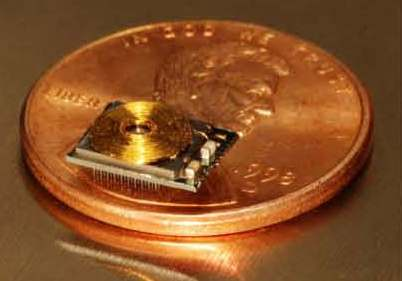
\includegraphics[width=6cm]{./0_intro/img/FSolzbacher01.jpg}
    \caption{Power System in a Package buck converter.}
    \label{fig:psoc_example}
\end{figure}

Besides the size reduction that an integrated driver would offer, such an approach would also bring other benefits in terms of control and connectivity.  The power management unit and driver control unit could be integrated together, providing the necessary intelligence for light control and the connectivity optimized for the requirements of the coming connected lighting industry. \emph{Smart lamps} are a clear example of the requirements of the so called \emph{smart drivers}. The \emph{smart lamps} are wireless connected to a network providing remote control for the light intensity level and color from a web interface, a mobile application or a dedicated remote control. The internal electronics has normally four LED drivers - one per each color channel: red, green, blue and amber - and, at the same time, a wireless interface. The electronic board is populated with discrete power drivers and micro-controller units. A solution capable to integrate all the functions in a single IC, or few ICs (one per channel), will definitely reduce packaging and assembling costs and still providing the same functionality. At the same time, the expected market volume for SSL technologies will, with no doubt,  justify costs of a dedicated ASIC design for LED drivers. All-in-all it has been the goal of this PhD thesis with the goal to explore and identify new architectures suitable for  integration that can efficiently power LEDs. The rational to explore the architectures that enable high density highly miniaturized power LED drivers, such as switched capacitor converters, developing a design framework based on a model-centric approach.



\bibliographystyle{plainnat}
\bibliography{references} 